\chapter{Introduction}
\pagenumbering{arabic}

%\section{Video Codecs}
Video is the dominant traffic type on mobile networks today and is expected to take up 70\% of all traffic in a few years. To effectively store and transmit high-quality video the data needs to be encoded. Modern video coding algorithms can decrease the size of raw video by hundreds of times with little or no discernible loss in video quality. To achieve this, local redundancies within each frame and between neighboring pictures are utilized, and different statistical methods guide the process to achieve the lowest file size at the least distortion of picture quality.

The standard scenario for digital video is for the images first to be captured by a camera, then encoded and stored somewhere, and transmitted over a network. On the receiving end the process is reversed; the sequences is decoded and then displayed. An encoder always goes together with a decoder, together the two are known as a \textit{codec}~\cite{Vcodex_Introduction_to_Video_Coding}.


\section{Image and Video Fundamentals}

\subsection{Digitally Representing Images and Video}
The simplest form of image, a greyscale one, can be represented as a \textit{light intensity function}~\cite{Wien_Coding_Tools}. The intensity function exists in continuous space and has infinite precision. For every x- and y-coordinate there is a light component representing the brightness of the image. To get a digital image from the light intensity function we \textit{sample} it at certain intervals. The samples are usually confined to a rectangular area -- the borders of the image. Light samples are called pixels or pels, from the word \textit{picture element}. The number of samples in a frame are usually written in the form $N \times M$ giving the number of horizontal versus vertical samples~\cite{Flierl}, for example $1920 \times 1080$. It is also common to refer to the frame size only by its height.

What sets video apart from still images is movement. Several images shown in rapid succession creates the illusion of movement as long as the \textit{frame rate} is at least 24 \gls{fps}~\cite{Wien_Coding_Tools}. Higher frame rates give a smoother-looking video, so many systems use frame rates around 50-60 \gls{fps}. \Gls{hd} or Ultra HD content will often have frame rates ranging from 100 to 200 \gls{fps}.

\subsection{RGB, YCbCr and Chroma Subsampling}
\label{subsec:subsampling}

\begin{figure}
    \centering
    \includegraphics[scale=0.25]{pictures/wikipedia/public-domain/rgb-to-ycrcb.png}
    \caption{RGB to YCbCr conversion}
    \label{fig:rgb_to_ycbcr}
\end{figure}

A light intensity function represents a greyscale image. To represent color we sample the light at different frequencies and then display the components together. Classically \gls{rgb} are sampled which suffices to represent any color on the human visual spectrum~\cite{Flierl}. However, in most modern applications, \gls{rgb} is transformed to the \gls{ycbcr} format. Here Y is the \textit{luma} component, representing the overall brightness of the image, and Cb and Cr are \textit{chroma} components, representing intensity in blue and red~\cite{Wien_Coding_Tools}, see \cref{fig:rgb_to_ycbcr}.

Because the human eye is more sensitive to light than color~\cite{Vcodex_Introduction_to_Video_Coding,Wien_Coding_Tools}, in \gls{ycbcr} the two color components are usually \textit{subsampled} so that chroma values are averaged from a neighborhood of pixels, and subsequently less information is transmitted for the chroma than for luma~\cite{Flierl}. This subsampling is conventionally written as a ratio between luma and chroma samples $$Y:X_1:X_2$$ with $Y = 4$ in most applications. $X_1$ describes horizontal subsampling, so $X_1 = 2$ means that 2 chroma samples are taken horizontally for every 4 luma samples. $X_2$ describes the vertical subsampling in relation to $X_1$. $X_1 = 0$ indicates that the same chroma subsampling is performed vertically as horizontally, while $X_1 = 2$ indicates no vertical subsampling is performed That is, the number of chroma samples are the same as the luma samples. See \cref{fig:subsampling_ratios}. $4:2:2$ and $4:2:0$ are the most common subsampling formats~\cite{Wien_Coding_Tools}.

In $4:2:0$, for every $2 \times 2 = 4$ luma pixels, only 1 pixel is stored in the two chroma components, meaning that a $1920 \times 1080$ video subsampled at $4:2:2$ contains only $960 \times 540$ chroma samples. Naturally, this decreases the size of the stored video. One full luma sample plus two chroma components each a one fourth of the luma size give a total of 1.5 samples, as opposed to the 3 full samples needed in \gls{rgb}. Done correctly, chroma subsampling has little to no effect on the resultant video, and instead for the same file size as without subsampling the overall resolution and quality can now be increased.

\begin{figure}
    \centering
    \copyrightbox[r]
        {\includegraphics[scale=0.5]{pictures/wikipedia/creative-commons/Chroma_subsampling_ratios.pdf}}
        {\textcopyright{ \href{https://en.wikipedia.org/wiki/File:IPB_images_sequence.png}{Image by Brion VIBBER and Mysid / CC BY-SA 3.0}}}
    \caption{Different subsampling ratios}
    \label{fig:subsampling_ratios}
\end{figure}

But even with \gls{rgb} transformed to \gls{ycbcr}, storing or transmitting each pixel value is expensive in terms of storage space and bandwidth. 10 seconds of $4:2:0$ video content with 8 bit intensity values at $1920 \times 1080$ resolution and 50 \gls{fps} will require $1.5 \,\times\, 10 \,\times\, 8 \,\times\, 1920 \,\times\, 1080 \,\times\, 50 \, \text{bits}= 1.6 \, \text{GB}$ of data. A two hour movie requires 1.1 TB. This is why we need video compression.

\subsection{Binary Numbers}
\label{subsec:binary-numbers}
To store and transmit data in any computer system, numbers are converted to \textit{binary} format. Instead of ten digits, 0--9, binary deals exclusively with two numbers: 0 and 1. These can be more easily represented digitally. Both the decimal and binary systems gives significance to digits based on their position within the number. This is called a positional system. Take the decimal number 312, which can be re-written as $$3 \times 100\, + 1 \times 10\, + 2 \times 1$$ which furthermore can be written as $$3 \times 10^2\, + 1 \times 10^1\, + 2 \times 10^0$$

The internal logic of numbers is so ingrained into everyday thinking that we usually never need to worry about it, but binary conversion forces us examine the internal logic of a positional system. Because binary only has two digits, each positional exponent is now a 2 instead of a 10. 312 would in binary be represented as $$1 \times 2^8\, + 0 \times 2^7\, + 0 \times 2^6\, + 1 \times 2^5\, + 1 \times 2^4\, + 1 \times 2^3\, + 0 \times 2^2\, + 0 \times 2^1\, + 0 \times 2^0$$ which is equal to $$1 \times 256\, + 0 \times 128\, + 0 \times 64\, + 1 \times 32\, + 1 \times 16\, + 1 \times 8\, + 0 \times 4\, + 0 \times 2\, + 0 \times 1$$ and which we write as as $100111000_{2}$. We use subscript to signal the number base, but this is usually left out when it is clear from context what number domain we are in. The conversion itself is non-trivial, and we won't go into detail on how to actually convert $312_{10}$ to $100111000_{2}$. However, it can easily be verified that the binary sum above sum indeed adds up to the expected value, and it can furthermore be proven that every binary representation is unique.


\section{Encoding Fundamentals}

A video encoder is a program that takes some form of raw video and produces a \textit{bitstream}, a sequence of bits, 0's and 1's. The encoder does this by going over the video frame-by-frame, often in a non-sequential order, using a multitude of algorithms to codify and store information using as few bits as possible. The decoder then turns the bitstream into pixel data again. \Gls{hevc}, like most video coding standards, only specifies the behavior of its decoder. That is, a bitstream is said to conform to the \gls{hevc} standard as long as it can be decoded by its decoder, regardless of the quality of the video output. The implementer of an encoder is free to make choices about the coding as long as the resulting bitstream conforms to the standard -- which naturally limits the freedom.

A certain portion of the encoding is \textit{lossless}. That is, information is repackaged in a form so that it can be completely restored by the decoder~\cite{Flierl}. This is done by exploiting statistical redundancies within the data. Arithmetic coding presented below is an example of lossless coding. Although the idea is obviously attractive, the potential gains from using only lossless encoding are far to small to be effective which is why lossy coding techniques are generally employed as well. Usually both are used together.

In \textit{lossy} compression data is irreparably distorted. A good coding algorithm achieves large decreases in file size without sacrificing too much quality, and any decrease in bit rate is always weighed against the quality loss it introduces. Lossy coding techniques exploit not only statistical redundancies but also visual ones; things that look similar in a frame can be coded together to save space. The aim of the process is to remove information that in not visible to the human eye, while leaving most of what is visible~\cite{Flierl}. Depending on the application, we may chose a smaller file size but with clear visual artifacts and distortions, and other times we want a compressed a image that looks almost identical to its original. Both are possible using lossy compression.


\begin{figure}
    \centering
    \includegraphics[scale=0.4]{pictures/wikipedia/public-domain/Point_quadtree.pdf}
    \caption{Quadtree splitting}
    \label{fig:quadtree}
\end{figure}

%\subsection{Partitioning}
%\begin{figure}
%    \centering
%    \includegraphics[scale=0.4]{pictures/vcodex/introduction-to-high-efficiency-video-coding/CUs}
%    \caption{A slice outlined in blue, and quadtree splitting all across the frame}
%    \label{fig:quadtree}
%\end{figure}

The first step of the encoding process is partitioning. The \gls{hevc} encoder divides the frame into slices that can be encoded in parallel, this is usually done once for the whole sequence. Then each slice goes through \textit{quadtree} partionining. The slice is divided into $64 \times 64$ \glspl{ctb}~\cite{Vcodex_HEVC_introduction}, which are then recursively split into four equally sized subsections (see \cref{fig:quadtree}). Both options -- splitting and not splitting -- are performed, the area encoded and the results are then compared to decided whether to continue splitting or to stop. For every split, this procedure is repeated for each of its four subsections, and each block can be split over and over again until minimum block size of $8 \times 8$ is reached~\cite{Van_Wallendael}. Areas with sparse movement are easier to compress and will generally not be divided as much, forming larger continuous sheets in the quadtree structure~\cite{Vcodex_HEVC_introduction}.

\subsection{Prediction}
To radically cut down on the amount of information that needs to be stored, we usually try to generate a prediction of the image, which we then subtract from our frame and then we work with this residual instead. The prediction needs to be done in such a way that the decoder can reliably reverse the process and recreate the image. This means that only data that has already been encoded can be used for further predictions, because this is what will be available to the decoder at the corresponding point in the decoding process.

Although the encoder has easy access to the whole sequence, it limits its predictions to what it previously encoded to allow the content to be decoded. Of course, if the decoder cannot decode what has been encoded then the bitstream is worthless.

%\begin{figure}
%    \centering
%    \includegraphics[scale=0.6]{pictures/vcodex/introduction-to-video-coding/prediction}
%    \caption{Prediction of a frame and the residual}
%    \label{fig:prediction-residual}
%\end{figure}

\subsubsection{Intra Prediction}
One prediction technique focuses on the internal relations between blocks in a image and is called \textit{intra prediction}. Textures in a non-random image tend to look like each other~\cite{Wien_Coding_Tools} -- if you zoom in enough on any structure in an image, many close-by pixels hold the same or similar color values -- so the assumption is that a decent prediction can be generated by approximating blocks by their closest neighbors. The intra prediction concept is shared between still image and video compression.

%\Cref{fig:jpeg_intra_prediction} depicts the prediction of pixel X using the values for neighboring samples A, B, C and D. Notice how no information from below or to the right of the pixel is utilized. The encoder moves in a pattern row-wise from left to right, so those values have not yet been encoded.

%\Cref{fig:intra_prediction} depicts the prediction of one block using the pixels values from the previously encoded blocks to its left and above it. The different sub-images show different modes. Generally the encoder tries each one and settles on the one that gives the best prediction. The mode is then signaled in the bitstream so that the decoder can replicate the prediction and reverse the process.

%\begin{figure}
%    \centering
%    \includegraphics[scale=0.6]{pictures/naver/intra-prediction}
%    \caption[hej]{Intra prediction with different modes}
%    \label{fig:intra_prediction}
%\end{figure}

Most of the information in the residual of an intra predicted frame will be contours of shapes in the picture~\cite{Vcodex_HEVC_Walkthrough}, as those are hard to predict using this method.

\subsubsection{Inter Prediction}
A more powerful prediction technique for video content uses differences between frames and is called \textit{inter prediction}. The basic assumption here is that objects within an image will appear in multiple frames but will move around. If an object from a previous frame can be identified and followed then this information can be used to make accurate predictions, see \cref{fig:inter_prediction}.

\begin{figure}
    \centering
    \includegraphics[scale=0.6]{pictures/wikipedia/public-domain/Interframe_prediction_cropped.png}
    \caption{Inter prediction}
    \label{fig:inter_prediction}
\end{figure}

Identifying an object from one frame to another means that a search has to be performed. This is a computationally complex process. While it is not impossible to search the whole frame for a best match, for any higher resolution video it is often unrealistic to do so and generally the search is confined to some nearby region of the previously known position~\cite{Wien_Coding_Tools}. Using a \gls{mse} calculation~\cite{Flierl}, the closest match is identified, and a \gls{mv} is stored in the bitstream to signal the displacement from one frame to the next. By storing \glspl{mv} instead of pixel data, we avoid duplicating data from previous frames and can once again cut down the information content of the resulting file~\cite{Flierl}. Calculating motion vectors is the most expensive part of encoding, especially because of the wealth of options offered by \gls{hevc}~\cite{Van_Wallendael}.

For both prediction techniques we won't generally achieve a perfect match, and the residual will contain our prediction error. However, our expectation is not generally to reduce the residual to nothing, only to make it as small as we possibly can. Using the residual data together with our prediction information we could still generate a perfect reconstruction of the encoded sequence. It is not until a later step that we start introducing distortion in the frame.

\begin{figure}
    \centering
    \copyrightbox[r]
        {\includegraphics[scale=0.3]{pictures/wikipedia/creative-commons/Sintel_Motion_Vectors.png}}
        {\textcopyright{ \href{https://en.wikipedia.org/wiki/File:IPB_images_sequence.png}{Image by Blender Foundation / CC BY 3.0}}}
    \caption{Motion vectors superimposed on the frame}
    \label{fig:motion_vectors}
\end{figure}

%The residual is calculated by taking pixel values of the referenced frame and shifting them according to the motion vectors. Then the prediction is subtracted from the actual frame, and this is what is passed on to the next step of the encoding. Again, we heavily cut down on the information content that we need encoded, but no information is irreversibly lost. Without the quantization step, the process would be fully reversible; the residual added back to the prediction and the effects of the motion vectors reversed.

%When a sequence is encoded using inter coding, only certain frames or areas within frames will contain residual data for the actual picture content. Most of what we store is motion data together with references to one or several other frames. Thus, an inter coded frame cannot be decoded without first decoding the frames that it references. Depending on how good the prediction is -- in a scene change, for example, it will generally be very bad -- the residual will end up containing very little information.

As opposed to intra-prediction, contours of stationary objects will mostly disappear from the inter prediction, and what is left are areas with hard-to-predict movement~\cite{Vcodex_HEVC_Walkthrough}. Accurate \glspl{mv} give better prediction, but come at a certain signaling cost. \Glspl{mv} usually have an accuracy ranging from one pixel to a quarter pixel, so the vertical and horizontal displacements are correct up to one fourth's of a pixel's size~\cite{Wien_Coding_Tools,Flierl}. See \cref{fig:motion_vectors} for motion vectors superimposed on a frame.

\subsubsection{Rate-Distortion Optimization (RDO)}
\label{subsec:rdo}
It is up to the encoder to chose whether to encode each section of a frame using intra or inter prediction~\cite{Wien_Coding_Tools}. This is decided dynamically using techniques like \gls{rdo}~\cite{Sullivan}, shown in \cref{eq:rdo}. $D$ stands for distortion, $R$ stands for bit rate and $\lambda$ is a weight parameter that can be arbitrarily assigned to steer the encoding in a certain direction. We encode each option and chose the one with the lowest $J$, that is, the choice with the lowest distortion to relative the rate.

\begin{equation}
\label{eq:rdo}
J = D * \lambda + R
\end{equation}

%\begin{figure}
%    \centering
%    \includegraphics[scale=0.6]{pictures/Flierl/09-RDO}
%    \caption{An RDO graph}
%    \label{fig:rdo-graph}
%\end{figure}


\subsection{Frequency Transformation and Quantization}
\label{subsec:quantization}
After partitioning and prediction, each block is frequency transformed using \gls{dct}~\cite{Sauer}, and then \textit{quantized}. There exist a number of similar versions of \gls{dct}, but in image and video compression we generally use DCT-II, shown in \cref{eq:dct}~\cite{Flierl}.

%This pair is thus often referred to as \textit{the} \gls{dct}~\cite{Wien_Coding_Tools}.

\begin{equation}
\label{eq:dct}
X_k = \sum_{n=0}^{N-1} x_n \cos \left[\frac{\pi}{N} \left(n+\frac{1}{2}\right) k \right] \quad \quad k = 0, \dots, N-1.
\end{equation}

\begin{figure}
    \centering
    \includegraphics[scale=0.55]{pictures/wikipedia/public-domain/quantized-signal.pdf}
    \caption{Quantization thresholds}
    \label{fig:quantization-thresholds}
\end{figure}

Quantization means rounding the coefficients to some preset levels, decreasing the information content and allowing us to store the video at a decreased size. See \cref{fig:quantization-thresholds}. We specify a \glsfirst{qp}\glsunset{qp} to set the coarseness of the quantization, where a lower \gls{qp} means less rounding. The quantization process introduces an irreversible distortion to the frame so that the original values cannot be recovered~\cite{Wien_Coding_Tools}.

By its nature, a frequency transform divides the coefficient by their frequency content, low-frequency components are in the top-left corner and higher-frequency toward the bottom-right. The low-frequency components correspond to contours in the image and high-frequency components generally correspond to details. We utilize the fact that lower-frequency components are more visible to the human eye and thus use a higher \gls{qp} for the higher-frequency components, effectively low-pass filtering the matrix~\cite{Sauer}. Adjusting \gls{qp} values allows us to specify exactly much degradation we are willing to accept in order to save bit rate -- file size is traded for visual accuracy.

\subsection{Arithmetic Coding}
\label{subsec:arithmetic-coding}
The reason why quantization actually makes our files smaller is because we later encode sequences in a way so that shorter and more frequent numbers take up less space. In the pixel domain, using 8 bits, each value take up the same amount of bits, so 0 for example is represented as 00000000, which is wasteful.

\begin{figure}
    \centering
    \includegraphics[scale=0.3]{pictures/wikipedia/Arithmetic_encoding}
    \caption{Arithmetic coding}
    \label{fig:cabac}
\end{figure}

Arithmetic coding is a lossless compression method where a string of symbols is encoded as a fraction in the interval $I=[0,1)$. By using the probabilities of each symbol and recursively subdividing $I$, we eventually get a sub-interval uniquely representing our string (see \cref{fig:cabac}). By encoding the length of our original sequence and by then calculating a binary fractional expansion residing completely within the interval, we can uniquely reverse the process to decode our message. \gls{hevc} performs arithmetic coding using an algorithm called \gls{cabac}~\cite{Vcodex_HEVC_introduction}, that was first introduced in \gls{h264}.

\subsection{GOPs and Temporal Layers}
\label{subsec:gops-and-temporal-layers}
Encoded frames are divided into categories based on how they interact with other frames. Intra coded frames are called I-frames and they appear at the start of a sequence and at certain set points to allow the video to be decodable without having to always start the decoding from the very beginning. Most frames are predicted from other frames and are called P or B-frames. A P-frames uses one other frame for its prediction and a B-frame use two, usually one before and one after itself. See \cref{fig:frame_types}.

\begin{figure}
    \centering
    \copyrightbox[r]
        {\includegraphics[scale=0.7]{pictures/wikipedia/creative-commons/IPB_images_sequence.png}}
        {\textcopyright{ \href{https://en.wikipedia.org/wiki/File:IPB_images_sequence.png}{Image by Brostat\\CC BY-SA 3.0}}}
    \caption{Different frame types in a sequence}
    \label{fig:frame_types}
\end{figure}

An encoder divides the input video into \glspl{gop} when encoding. A \gls{gop} is treated as a unit by the encoder and can be usually be decoded independently from the rest of the video. This allows the viewer to skip ahead to any given time in the video without having to decode everything prior to it. While larger \glspl{gop} generally give better encoding performance~\cite{johan}, \gls{gop} sizes are generally chosen so that every second or half-second of video content is independently decodable.

%\begin{figure}
%    \centering
%    \includegraphics[scale=0.6]{pictures/Flierl/12-GOP}
%    \caption{A group of picture containing three frame types}
%\end{figure}

Inter-coded video is generally not encoded in the frame order that the material was captured in. We distinguish between \textit{output order} and the \textit{decoding order}~\cite{Wien_Coding_Tools}. The \gls{gop} structure specifies a coding order which is then repeated cyclically throughout the sequence~\cite{Wien_Coding_Tools}.

The \gls{gop} structure also divides frames into temporal layers~\cite{Wiegand}. Intra coded frames form temporal layer 0 because they depend on no other pictures. Those that reference layer 0 pictures form layer 1 and pictures that depend on layers 0 and 1 are temporal layer 2, and so on. A popular GOP structure, \textit{Randomaccess}, has 4 temporal layers. The \gls{qp} values are usually increased slightly for the higher temporal layers. The rationale is that these generally contain less data, so compressing them slightly more won't have much of an effect on the sequences as a whole.


\section{HEVC-Specific Algorithms}

\subsection{RDOQ}
\Gls{rdoq} is a method for improving coding efficiency by manipulating transform coefficients after quantization. Out of the available quantization levels, we try different values and perform \gls{rdo} to decide the best value to re-assign each coefficient. Testing all possible combinations of quantization steps and coefficients in for example a $16 \times 16$ matrix would very computationally heavy so instead we go through the matrix one coefficient at a time from the bottom-right and backwards, setting each on the all possible levels or just a subset of its closest neighbor values.

\subsection{Sign-Bit Hiding}
\Gls{sbh} is a lossy technique for decreasing bit rate. To avoid transmitting the sign for the top-left element in a block of transform coefficients, it is instead inferred from the parity of the sum of all coefficients. Because transform coefficients are represented in binary form, and all even binary numbers numbers end with 0 and all odd ones end in 1, only the last bit of each coefficient needs to be taken into account.

Assuming that coefficients are equally likely to be even as odd, this parity is going yield the incorrect result half the time. To counter this, the \gls{sbh} algorithm performs \gls{rdo} over the transform block to find the value that would have the least impact on the resultant image if changed up or down by one, and then performs this change. That is, in order to save one bit on every transform block, a small error in introduced in half of the encoded blocks. The result is typically well worth it. Small losses in quality are traded for larger decreases in bit rate.

%As opposed to \gls{rdoq}, the decoder needs to be aware of \gls{sbh} so it is signaled in the sequence header.



\section{Adaptive Streaming}
\label{sec:adaptive-streaming}
Streamed video-on-demand content is usually delivered using \gls{abr}~\cite{Rusert}. Depending on device capabilities and bandwidth, different users will request different-quality content. A user that starts out watching a video when bandwidth usage is low will generally be sent high-quality video. If the available bandwidth then decreases -- maybe by more users entering the network -- the streaming service needs to dynamically lower quality to alleviate the network. \gls{abr} means that the transmitted quality is adapted to the receiver's needs.

Video cannot be downscaled in encoded form. Thus, to create a lower-resolution encoding of a video, it has to be decoded, downscaled and then re-encoded. This process is known as transcoding. The encoding step takes a lot of time, so to be able to do adaptive streaming, the service generally creates all encoding beforehand and stores them until they need to be transmitted. %This will naturally take up a certain amounts of space.

%[In a realistic scenario, a number or storages for original video and side-information are placed in urban areas. Hubs are then placed in large numbers, close to end-users. From the storage areas, originals and side-information can be sent over to a hub at the first instance any user requests it, it is then stored at the hub for a certain amount of time depending of the demand, and then reconstructed on-the-fly when the end-user wants to watch the video.]

We present here three models for adaptive streaming: simulcasting, \gls{jit} transcoding and \gls{svc}, and discuss their respective weaknesses. In the next chapter we will introduce \gls{gt} as way to get around some of the inherent problems of the current streaming models.

\subsection{Simulcasting}
The straightforward way create adaptive video content is that whenever a new video is ingested in the \textit{adaptation node}, we scale it to each desired size and encode (see \cref{fig:simulcasting}). The original video is then thrown away.

\begin{figure}
    \centering
    %\includegraphics[scale=1.2]{pictures/rusert/simulcast}
    \includegraphics[scale=1.2]{pictures/visio/simulcast}
    \caption{Simulcasting}
    \label{fig:simulcasting}
\end{figure}

This model is known as upfront transcoding or \textit{simulcasting}~\cite{Rusert}. A streaming service offering 1080p, 720p, 540p and 360p versions of all of its content will have one encoding for each resolution stored away and ready for transmission. This takes up a lot of space~\cite{Van_Wallendael}, and encodings are generated without prior knowledge of customer demand.

\subsection{Just-in-Time Transcoding}
\label{subsec:jit-transcoding}
The problem with simulcasting is that we may end up storing many files that are seldom or never actually requested~\cite{Rusert}. A more attractive idea might then be to encode the original only at the highest resolution, and later transcode it to the lower resolutions on-demand (see \cref{jit-transcoding}). The generated lower-resolution encodings may be kept as long as demand is high and then thrown away. This model is known as \gls{jit} transcoding.

\begin{figure}
    \centering
    %\includegraphics[scale=1.2]{pictures/rusert/jit-transcoding}
	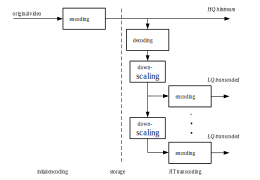
\includegraphics[scale=1.2]{pictures/visio/jit_transcoding}
    \caption{Just-in-time transcoding}
    \label{jit-transcoding}
\end{figure}

The general problem with \gls{jit} transcoding is that encoding takes a lot of time to perform. Even with specialized hardware, the process of encoding thousands of frames is generally too slow for the idea to work in practice~\cite{Rusert,Van_Wallendael}. Unless encodings can be generated within minutes, \gls{jit} transcoding is not appropriate for video streaming. For example, the idea or ordering a movie at 540p and having to wait a day for the content to be available would likely scare away most costumers in a world where proper on-demand streaming already exists.

Another problem with \gls{jit} transcoding is that the lower-resolution content will be generated from an already-degraded data source. In simulcasting, each encoding is generated directly from the original, but now the highest-resolution encoding acts as an original for the transcodings. This introduces \textit{generation loss}; coding artifacts and high-resolution noise that are amplified by successive transcoding, and lowers the video quality~\cite{Vetro}, as well as unnecessarily increasing its size. This problem is shared with our pruning approach to \gls{gt} (see \cref{sec:pruning}).

\subsection{Scalable Video Coding}
\Glsfirst{svc} uses a layered model to encode different-quality representations of the same material. Starting with a base layer, which is a regular bitstream, one or several enhancement layers are encoded with reference to the base. Enhancement layers can only be decoded after first decoding the base layer. Often, the different layers represent varying resolutions, with the base layer holding the lowest resolution and each enhancement layer representing a higher resolution.

Decoding a higher-resolution \gls{svc} layer requires access to the base layer together with every intermediate enhancement layer. Decoding an enhancement layer means the previous layer is decoded, upscaled to the size of the enhancement layer and used for prediction. The process in repeated for every subsequent layer until the target resolution is reached. The term \gls{svc} stems from the \gls{h264} standard and is often known as \myacr{shvc} in \gls{h265}, but we will use the terms interchangeably and refer to both as \gls{svc}.

%[Find pyramid image]

The major problem with \gls{svc} is that the dependent structure causes a size overhead when encoding the enhancement layers. While storage space can be saved on the adaptation node compared to simulcasting, any higher-resolution videos transmitted to the customer will typically take up more space in \gls{svc} than in a regular encoding~\cite{Van_Wallendael}. \Gls{svc} generally performs better at the lower resolutions -- for example, adding a new lowest-resolution encoding to the scheme moves every enhancement layer further away from the base and actually lowers coding efficiency. As such, the whole idea of \gls{svc} is in many ways out of step with the modern usage were the demand is on HD, Ultra HD, and beyond.


\section{My Contributions}
The idea of guided transcoding is not a novel one. \cite{Van_Wallendael} explores pruning as an idea and compares it to simulcasting, \gls{jit} transcoding and \gls{svc} for a single lower-quality representation. No mention, however, is made of any partial techniques.

We expanded these experiments to a large scale with our simulation environment, where we test a wide array of downscaled sizes and \gls{qp} values, as well as using a work-around to be able to simulate the effects of \gls{sbh}. Deflation as an idea is presented for the first time in this thesis report.

Partial pruning and deflation were presented to me on the conceptual level by my Ericsson supervisors. I then implemented the bit manipulations in low-level C and also wrote thousands of lines of Python to run simulations and to automatically export the results to Excel sheets.